\chapter{Antecedentes y estado del arte}
\label{chapter:antecedentes}

\section{De la astronomía a la astroinformática}

En la actualidad nos enfrentamos a una avalancha constante de datos de creciente calidad y cantidad. Esta abundancia de información ha elevado la importancia de la \gls{DM} y el \gls{ML} a niveles sin precedentes. El volumen de datos disponible es tan abrumador que su extracción y análisis ya no pueden depender exclusivamente de la capacidad humana \citep{hey2009fourth}. 

En el ámbito de la astronomía, este fenómeno no es una excepción, y entre los tipos de datos más relevantes para esta disciplina se incluyen los provenientes de extensos relevamientos \citep{shen2003size} y simulaciones cosmológicas de vanguardia \citep{pillepich2018simulating, schaye2015eagle}. En otras palabras, los astrónomos interesados en explotar las fuentes de datos deben adentrarse en conceptos como el aprendizaje automático, la identificación de patrones, la minería de datos y la reducción de la dimensionalidad; todas estas técnicas han sido agrupadas bajo la  disciplina conocida como Astro-informática \citep{borne_astroinformatics:_2010}.

Es importante destacar que la Astro-informática no opera en aislamiento, ya que la masividad de la información actual, ha dado origen a diversas subdisciplinas informáticas que se dedican a abordar la tarea de organizar, acceder, integrar y extraer información de un creciente conjunto de datos, con el propósito de proporcionar apoyo en la toma de decisiones \citep{fox2011rise}.

\section{Galaxias}

Como se menciona en la introducción, en este trabajo estamos interesados en las subestructuras de las galaxias, así que hemos decidido utilizar unos párrafos para explicar por qué es necesario realizar estudio en simulaciones.

Observacionalmente las galaxias se clasifican según su morfología en dos tipos principales:  galaxias elípticas, las cuales presentan una apariencia elipsoidal y galaxias espirales, que exhiben una forma discoidal con brazos espirales y en la región central presentan una componente esferoidal \cite{hubble1936realm}.

A modo anecdótico puede mencionarse que esta clasificación es conocida como ``Secuencia de Hubble'', y fue interpretada originalmente como una secuencia evolutiva. Puede observarse la secuencia completa en la Fig~\ref{fig:hubble}.

\begin{figure}
    \centering
    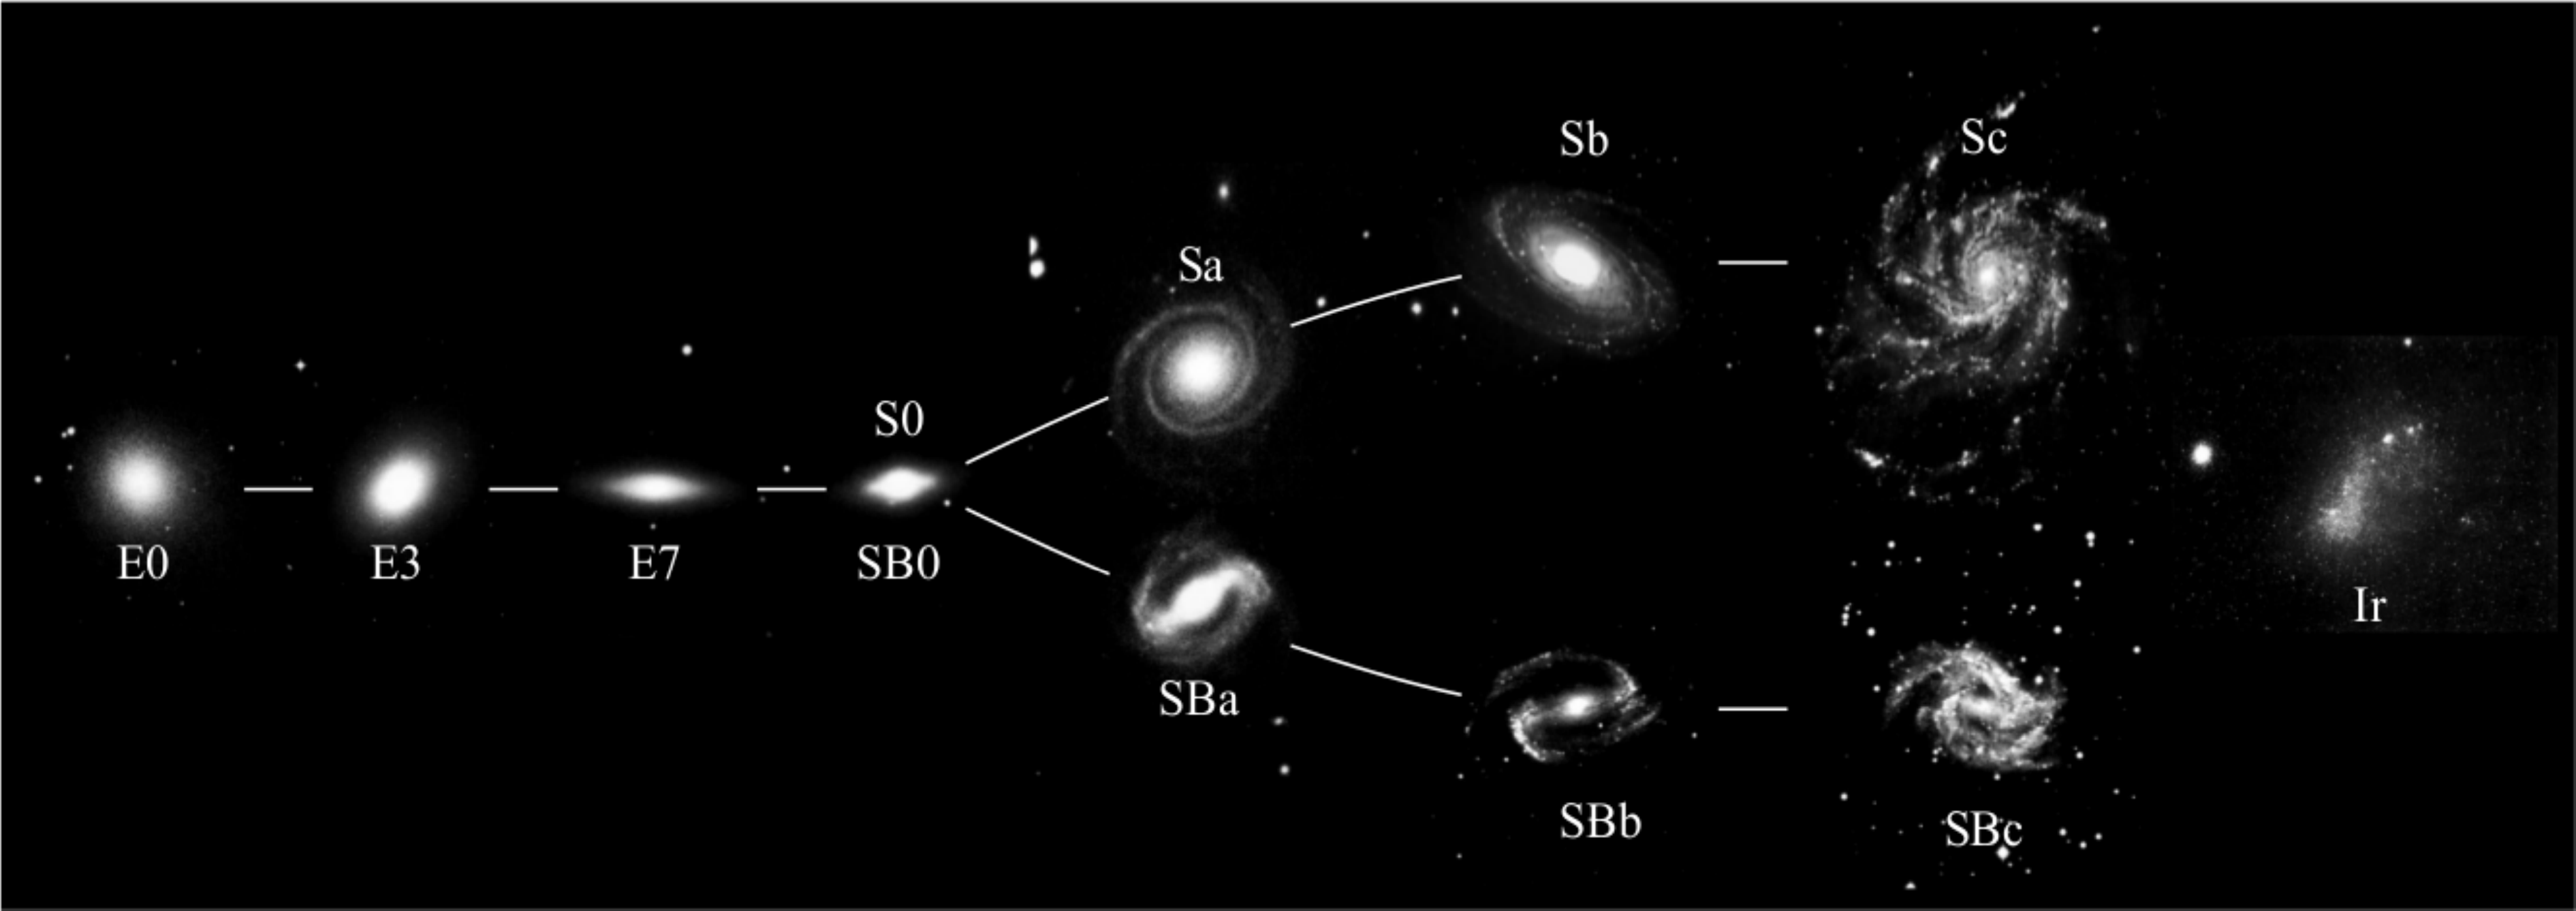
\includegraphics[width=.9\textwidth]{antecedentes/figures/hubble.png}
    \caption{\label{fig:hubble}  Clasificación morfológica o secuencia de Hubble \citep{carroll2006introduction}. En la rama principal izquierda pueden observarse arquetipos de galaxias elípticas (E0-E7), S0 es una lenticular, las ramas superior e inferior corresponde a galaxias espirales sin y con barra respectivamente. A la derecha una de tipo irregular.}
\end{figure}

Respecto a la estructura podemos destacar dos componentes estelares principales en las galaxias \footnote{Las galaxias además de estrellas poseen nubes de gas, polvo y materia oscura, elementos que están fuera del objeto de estudio de este trabajo.}:

\begin{itemize}
    \item El \textbf{esferoide} está compuesto por una población estelar roja y vieja, y, dependiendo el tipo de galaxia, éste puede ser más o menos prominente como el caso de las galaxias elípticas y espirales respectivamente. Además, se caracteriza por contener una baja cantidad de gas y polvo, resultando en una tasa de formación de estrellas relativamente baja \citep{mo2010galaxy}.

    Desde el punto de vista dinámico, las estrellas del esferoide se encuentran soportadas por dispersión de velocidades, aunque puede presentar una rotación mínima.

    Adicionalmente, se puede subdividir dicha componente en las subcomponentes llamadas Bulge y Halo.

    \item En el caso del \textbf{disco}, está compuesto principalmente por estrellas jóvenes, gas y polvo, los cuales se encuentran en rotación en un plano preferencial en torno al centro de la galaxia. Este es la componente principal de las galaxias espirales y lenticulares en lo que respecta a su masa. Además, el disco presenta una mayor tasa de formación estelar respecto al esferoide, debido a la existencia de gas en forma de hidrógeno, resultando en un color más azul gracias a la presencia de estrellas jóvenes. En particular, las galaxias espirales cuentan, como su nombre lo indica, con una estructura en forma de brazos espirales \citep{mo2010galaxy}.

    En galaxias de canto, se pueden identificar dos subcomponentes distintas: un disco delgado y otro grueso, con escala de radios similares, pero el primero es más delgado en altura y contiene generalmente poblaciones estelares más jóvenes, con un mayor contenido de gas frío y polvo que el segundo. Estos también son llamados ``Cold Disk'' y ``Warm Disk'' en la terminología en inglés, y utilizaremos ambas denominaciones de forma indistinta a lo largo del texto (en particular para referirnos a dichas subcomponentes en figuras, dado que estas siguen la terminología en inglés).
    
\end{itemize}

Es claro entonces que las galaxias son sistemas estelares complejos formados por varias componentes estelares que coexisten simultáneamente, las cuales definen su morfología y cinemática. Si bien queda claro que hay un estructura jerárquica, a lo largo de este trabajo dividiremos cada galaxia en cinco componentes: núcleo, disco fino y grueso, halo estelar y brazos espirales.

\subsection{Descomposición dinámica de galaxias y simulaciones}

Realizar una clasificación basada exclusivamente en la morfología de las galaxias tiene el problema de tener una influencia significativa de los efectos de proyección; ya que si consideramos una galaxia elíptica con semiejes $a > b = c$,  observadores diferentes situados en diferentes posiciones percibirán diferentes formas proyectadas de este objeto, como se ilustra en la Fig~\ref{fig:proyect}, y consecuentemente la clasificación variará en cada caso. El otro problema obvio que se presenta es que en proyección una estrella podría parecer que está en el esferoide mientras que en realidad está en el disco.

\begin{figure}
    \centering
    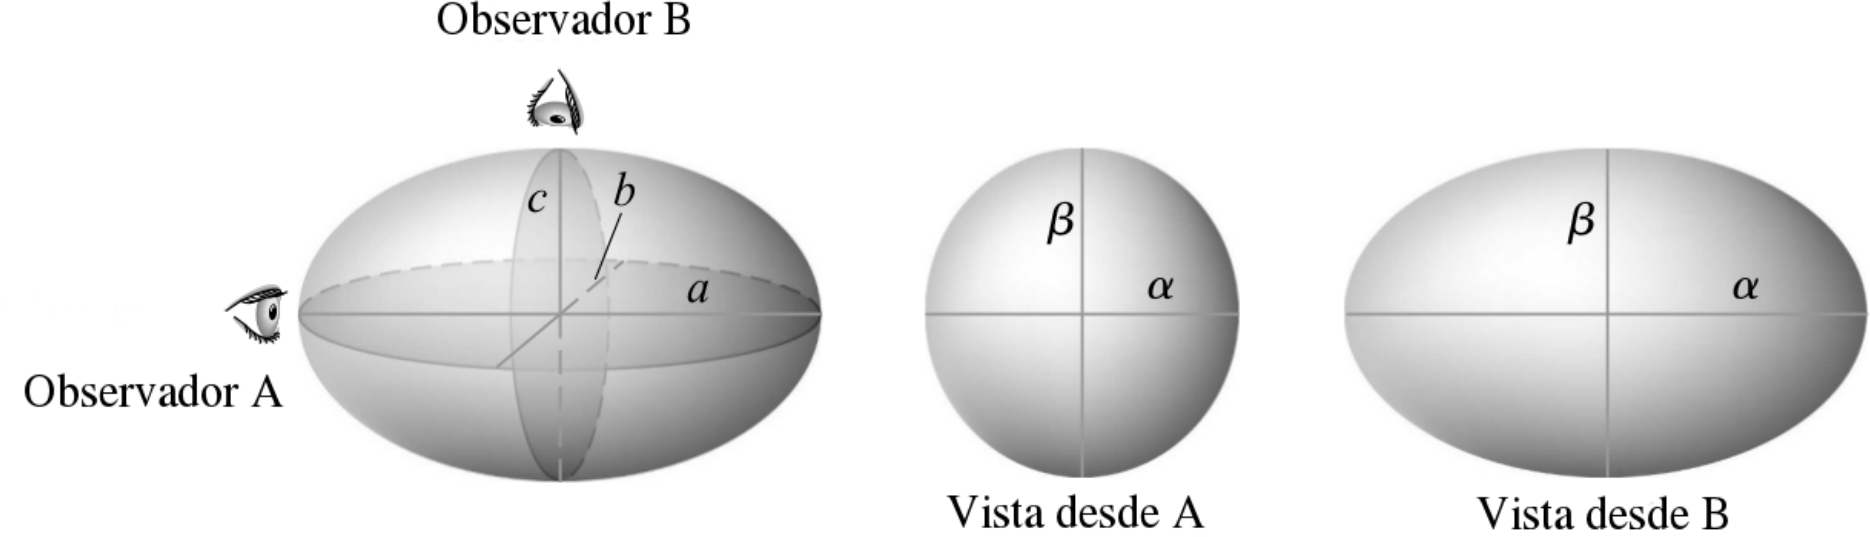
\includegraphics[width=.9\textwidth]{antecedentes/figures/proyecione_galactica.png}
    \caption{\label{fig:proyect} Proyecciones de una galaxia elíptica según la posición de dos observadores diferentes \citep{carroll2006introduction}}
\end{figure}

Así es que el campo de estudio ha enfocado sus esfuerzos en las características dinámicas de estrellas en las componentes, habiendo en la actualidad una amplia variedad de métodos para llevar a cabo la tarea de descomponer dinámicamente las galaxias. 

La naturaleza de este estudio requiere de disponer de las posiciones y velocidades de las estrellas individuales que la conforman, y esto excede a las capacidades observacionales de los telescopios actuales. En este sentido, las simulaciones hidrodinámicas cosmológicas de vanguardia existentes como EAGLE \citep{schaye2015eagle} y \gls{TNG} \citep{pillepich2018simulating} nos brindan la posibilidad de acceder a esta información. 

Estas simulaciones representan el estado del arte en cuanto a combinar una alta resolución numérica con volúmenes computacionales cosmológicos suficientemente grande para que incluyan decenas de miles de galaxias individuales. Típicamente cada una de estas galaxias está representada por decenas de miles de partículas que representan un elemento de masa del orden de $\sim 10^5 M_\odot$ (masas solares).

\citet{abadi2003simulations} fueron pioneros en esta área proponiendo el primer método para poder identificar las componentes estelares de una galaxia a partir de la distribución de lo que llamaron el parámetro de circularidad. Con el tiempo, surgieron diferentes variaciones del mismo, como los utilizados en los trabajos de \citet{governato2009forming, scannapieco2012aquila, tissera2012chemical, vogelsberger2014properties, marinacci2014formation} y \citet{park2019new}.

\subsubsection{Parámetros dinámicos y métodos}

Llegados a este punto  nos resulta importante definir qué parámetros son los que definen la dinámica de una partícula estelar en una galaxia. Así, los tres valores que representan los movimientos de una partícula estelar y definen su ubicación en alguna de las componentes son:

\begin{description}
    \item[Parámetro de circularidad ($\epsilon$):]

    Mide cuán parecida es la órbita de una partícula respecto a una órbita circular, para un dado valor de energía. Se calcula como el cociente entre la componente z del momento angular y el momento angular circular. Este último es el momento angular que tendría una partícula, si utilizase toda su energía cinética para moverse en una órbita circular.
    
\[\epsilon = \frac{J_{z}(E)}{J_{circ}(E)}\]

    \item[Parámetro de circularidad proyectada ($\epsilon_r$):] 

Representa la dispersión vertical del movimiento de una partícula con respecto al plano en el que se ubican las partículas que se mueven en órbitas circulares. 

    \[\epsilon_{r} = \frac{J_{p}(E)}{J_{circ}(E)}\]


Siendo  $J_P = \sqrt{J_x^2 + J_y^2}$, donde $J_x$ y $J_y$ son las componentes restantes del vector momento angular de la partícula estelar.
    
    \item[Energía estelar normalizada ($E/|E|_{max}$):]

    Es el cociente entre los valores de energía de las partículas estelares y el módulo de la energía de la partícula más ligada de la galaxia.

    Representa qué tan ligada está la partícula a la galaxia. Las partículas más ligadas al sistema van a adoptar valores cercanos a -1, mientras que las menos ligadas van a  tener valores cercanos a 0. Si el valor es cero la partícula se encuentra en una órbita parabólica mientras que  si es mayor a cero la partícula se encuentra en una órbita hiperbólica, en ambos casos éstas no se encuentran ligadas a la galaxia.

\end{description}

El espacio que define esta dinámica puede observarse en la Fig~\ref{fig:dyn_space}. Es claro que si bien se sabe que la dinámica de las partículas ubica a las componentes en diferentes zonas de la figura, sigue siendo un espacio muy denso donde no hay divisiones claras entre las componentes.


\begin{figure}
    \centering
    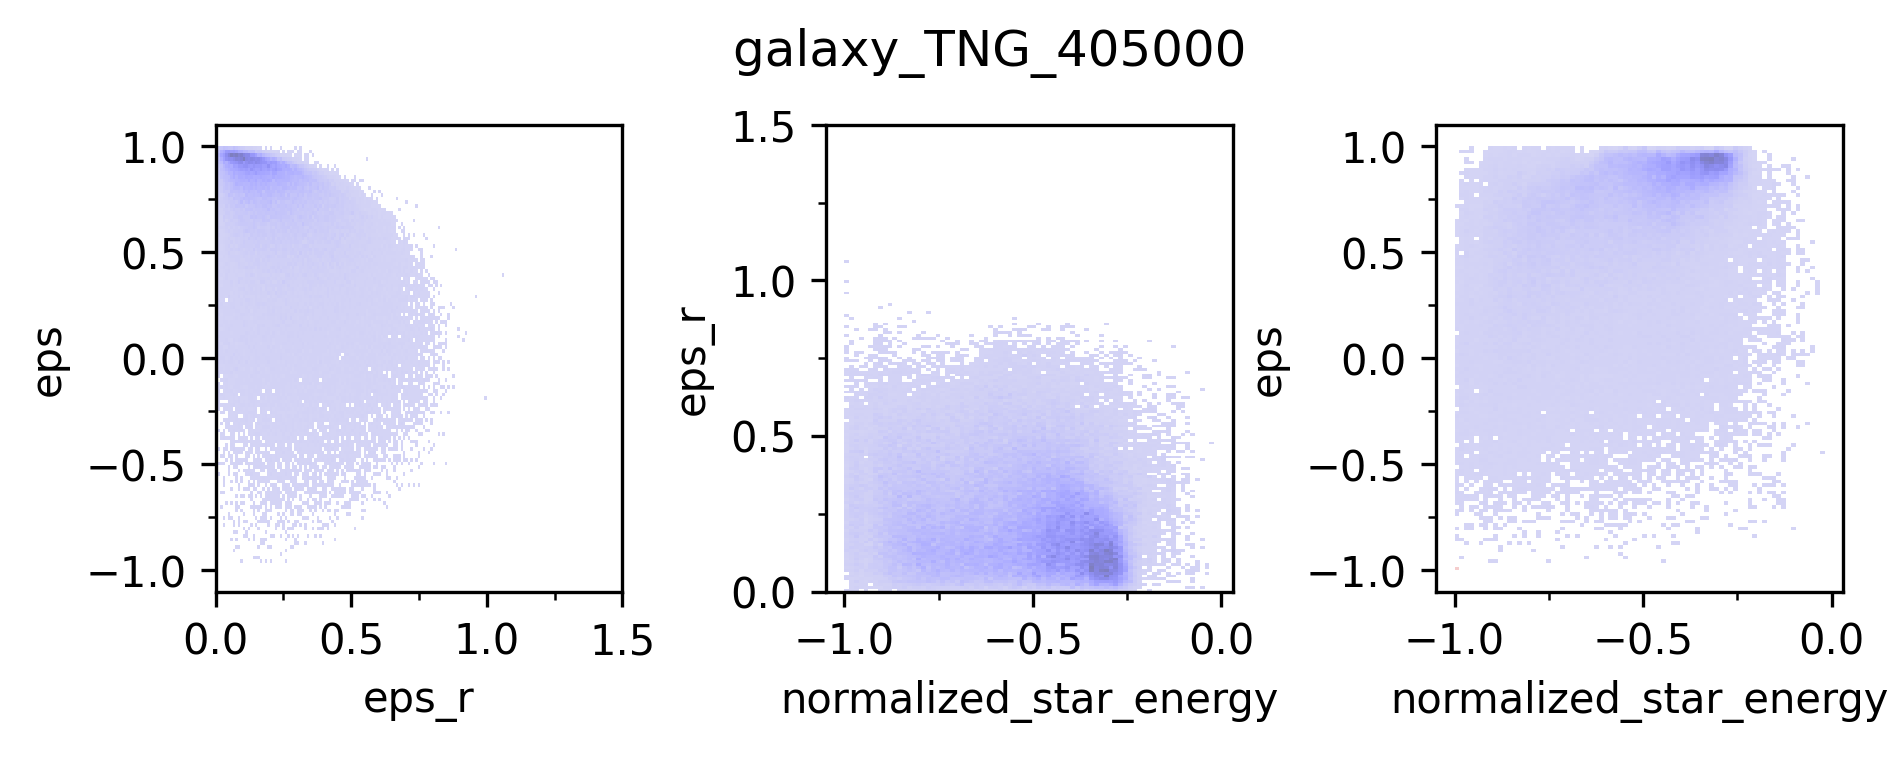
\includegraphics[width=.9\textwidth]{antecedentes/figures/dyn_space.png}
    \caption{\label{fig:dyn_space} Espacio dinámico de la galaxia TNG\_405000 en los tres parámetros de circularidad.}
\end{figure}

En los siguientes capítulos nos referiremos al parámetro de circularidad como $eps$, al parámetro de circularidad proyectada como $eps\_r$ y a la energía estelar normalizada como $normalized\_star\_energy$. Para, de esta manera, unificar la terminología utilizada en el código y la encontrada en los datos con este trabajo.

Una vez que hemos definido los parámetros, es el momento de establecer los métodos de descomposición dinámica que los utilizarán. En particular, nos centraremos en dos métodos que hacen uso de diferentes sub-conjuntos de los parámetros previamente definidos e identifican diferentes cantidades de componentes. 

\begin{description}
    \item[\citet{abadi2003simulations}:]

Utiliza el parámetro de circularidad $\epsilon$ definido anteriormente para separar las particulares estelares en dos componentes: el esferoide y el disco.

Este método asume que la componente esferoidal no presenta rotación y por lo tanto está representada por una distribución simétrica respecto de $\epsilon = 0$. Para ello selecciona el mismo número de partículas en órbitas corrotantes que aquellas que se encuentran en órbitas contrarrotantes. Luego, la distribución de las partículas restantes, se asignará al disco. Esto se debe a que el método asume que el disco está formado por partículas cuyo movimiento predominante es el de rotación. Como reflejo de esto, las partículas asignadas al disco tendrán $\epsilon \sim 1$.
    
    \item[\citet{du2019identifying}:] 

Realiza distribuciones Gaussianas que representan las estructuras a ser identificadas, utilizando $\epsilon$, $\epsilon_r$ y $E/|E|_{max}$ como las dimensiones de dichas distribuciones.

A su vez, genera modelos de dichas estructuras utilizando GMM (Gaussian mixture models), variando el número de componentes a buscar de 2 a 9. En cada iteración, se crean 10 modelos con diferentes inicializaciones para alcanzar resultados más estables.

El algoritmo usa una función a minimizar y un valor de disparo previamente establecido, de forma tal de terminar cuándo el resultado obtenido de esta función sea menor al valor de disparo. Como la iteración comienza con 2 grupos y crece desde ahí, se tiene preferencia en buscar pocas componentes.

El método no asigna ninguna significancia física a cada una de las componentes encontradas, derivando dicha tarea de interpretación al usuario.
    
\end{description}

Estos dos métodos nos servirán como puntos de referencia para comparar con los algoritmos que implementemos.

\section{Aprendizaje automático}

La actualidad nos ha brindado las computadoras como nuevas fuentes de conocimiento, al punto que como dice el director de investigación en inteligencia artificial de Facebook\footnote{\url{http://facebook.com}}, \textit{Yann LeCun}:

\begin{displayquote}
\textit{En el futuro, la mayor parte del conocimiento del mundo será extraído y almacenado dentro de máquinas.}
\end{displayquote}

Ese futuro predicho por \textit{LeCun}, es en realidad el presente y es el contexto en el cual la \gls{AI} se vuelve útil para aprovechar el poder de cómputo para que las maquinas auto--analicen su información. La \gls{AI} tiene diferentes ramas siendo la de éxito actual aquella que postula que se puede imitar la inteligencia humana por medio del aprendizaje. En otras palabras, podemos brindar datos de ejemplo a un programa para que entienda su ``forma'' y generalice en una tarea dada.

El \gls{ML} es una de las técnicas mas recurridas y exitosas en tiempos modernos dentro de la Astroestadística \citep{fluke2020surveying}. Puede encontrarse una de sus definiciones formales en el libro clásico del área ``\textit{Machine Learning}'' \citep{mitchell1997machine}:

\begin{displayquote}
Se dice que un programa de computadora aprende de la experiencia $E$
respecto a una tarea $T$ y una medida de desempeño $P$, si el desempeño medido con $P$ en una tarea $T$, mejora con la experiencia $E$.
\end{displayquote}

El \gls{ML} es un proceso inductivo para la exploración de conocimiento, donde su enfoque reside en la búsqueda de información general a partir de observaciones específicas que sesgan las suposiciones de conocimiento concreto, con el propósito de establecer una base sólida para realizar generalizaciones. 

El éxito de un método de \gls{ML} está dado por qué tan correctas resultan estas hipótesis y sesgos. Hay una preferencia particular por usar hipótesis simples, lo que suele llamarse ``\textit{Navaja de Ockham}''\footnote{\textit{Navaja de Ockham}: \textit{En igualdad de condiciones, la explicación más sencilla suele ser la más probable}. Así si dos teorías en igualdad de condiciones tienen las mismas consecuencias, es más probable que la teoría más simple sea la correcta.}

\subsection{Tipos de aprendizaje}

Todos los métodos de \gls{ML} comparten un rasgo fundamental: requieren datos de entrenamiento para adquirir conocimiento. Sin embargo, diversos tipos de tareas ($T$), experiencias ($E$) y desempeños ($P$) conducen a múltiples especializaciones. La clasificación inicial más común categoriza a los modelos de \gls{ML} en función de cómo el algoritmo utiliza o no valores objetivos a aproximar:

\begin{description}
    \item[Aprendizaje Supervisado] Busca lograr una aproximación adecuada de la función $F(X) = y$, en la que $X$ representa los datos de entrada o matriz de \textit{features} (características en inglés) y el vector $y$ corresponde a sus respectivas etiquetas o clases objetivos. Esta aproximación puede tomar la forma de un conjunto finito de etiquetas discretas (clasificación) o intentar predecir un valor numérico real que represente alguna magnitud (regresión).

    \item[Aprendizaje No-Supervisado] Adquiere conocimiento durante la ejecución de la tarea sin requerir etiquetas. Tareas de este tipo pueden abarcar la reducción de la dimensionalidad, la visualización de datos (manteniendo sus propiedades fundamentales) o la agrupación en conjuntos con características similares.
\end{description}

Sin importar el tipo de aprendizaje que utilicemos, la aplicación de estos algoritmos se separa en dos etapas: la de entrenamiento y la de predicción. En la primera se utilizan los datos de entrenamientos para ajustar los valores internos del modelo, luego de la cual  el modelo está listo para realizar predicciones sobre nuevas datos. Además, hay varios modelos que poseen hiperparámetros que pueden ser configurados previamente a la fase de entrenamiento.

Esta distinción de dos etapas del aprendizaje automatizado puede verse reflejada, por ejemplo, en los polinomios. En estos, la etapa de entrenamiento se basa en establecer los puntos del conjunto de entrenamiento como los coeficientes del polinomio (valores internos), siendo la etapa de predicción evaluar el polinomio. Este tipo de método es llamado ``Regresión Polinomial''.

Dado que las partículas estelares de las galaxias simuladas no poseen etiquetas sobre la componente galáctica a la cual pertenecen, este trabajo centrará sus esfuerzos sobre el aprendizaje no supervisado en general y el \textit{clustering}/agrupamiento en particular.

\subsection{\textit{Clustering}}

Como se mencionó en la sección anterior, es de nuestro interés aplicar métodos de agrupamiento o \textit{clustering}, para asignar las partículas estelares a las diferentes componentes galácticas. Así, los algoritmos de \textit{clustering} persiguen la tarea de agrupar un conjunto de objetos de tal manera que los objetos de un mismo grupo (llamado \textit{cluster}) sean más similares, en algún sentido, entre sí que los de otros grupos ($clusters$). Los algoritmos de esta familia tienen una taxonomía amplia y en este trabajo estamos interesados en tres tipos:

\begin{description}
    \item[Métodos jerárquicos: ] Estos métodos tienen la particularidad de crear agrupamientos basándose en agrupamientos más pequeños de una manera jerárquica.  
    
    Es esperable que este tipo de algoritmos representen de alguna manera la estructura jerárquica que exista dentro de las componentes galácticas \citep{johnson1967hierarchical}.

    \item[Métodos difusos/\textit{fuzzy}: ] Si bien técnicas de agrupamiento suave ya han sido aplicados al problema de descomposición dinámica como son los trabajos de \citet{obreja2018introducing} o \citet{du2019identifying}, no existen referencias respecto al uso de agrupamiento difuso. 
    
    Dado que una partícula de varias masas solares puede pertenecer a más de una componente galáctica al mismo tiempo, queremos evaluar cómo se comporta los métodos de agrupamientos basados en lógica difusa para la asignación de la misma partícula en diferentes componentes.

    \item[Métodos basados en acumulación de evidencia: ] Este tipo de métodos permite combinar y consensuar resultados provenientes de otras técnicas de clustering.
    
    Sabiendo la complejidad física encontrada en las galaxias, creemos que poder utilizar las mejores características obtenidas dentro de un conjunto de resultados puede resultar en una clusterización que no sería capaz de ser encontrada por ningún método individualmente.
    
\end{description}

Se expandirá sobre cada uno de los métodos mencionados en su capítulo correspondiente.

\subsubsection{Métricas externas}

Una característica que tienen los métodos de \textit{clustering} es que estos solo son capaces de discernir grupos entre sí, no catalogarlos. Por lo cual, una vez etiquetados los datos de cada galaxia, es necesario compararlos con los obtenidos con algún método que tengan una fundamentación física sólida y además provean estas etiquetas. A los resultados de estos métodos de referencia los consideraremos verdad de referencia o \gls{GT}.

Dado que nuestro interés radica en probar cómo los métodos antes presentados se pueden configurar para que encuentren diferentes números de grupos, hemos decidido utilizar como \gls{GT} los métodos de \citet{abadi2003simulations} y el de \citet{du2019identifying}, teniendo el cuidado de utilizar los mismos parámetros dinámicos para realizar el agrupamiento en cada caso. Así, por ejemplo, si el método de \citet{abadi2003simulations} sólo utiliza el parámetro de circularidad ($\epsilon$) y busca dos \textit{clusters} y deseamos compararlo con un método jerárquico, también utilizaremos solo $\epsilon$ y buscaremos como máximo dos \textit{clusters}.

Comparando los resultados obtenidos por el \gls{GT} y los del método que estemos evaluando, podemos crear la \gls{CM}, como la que se presenta en la Tabla~\ref{tab:conf_mtx}.

\begin{table}[]
    \centering
    \begin{tabular}{c|c|c}
         {}                   & \multicolumn{2}{l}{\hfil \textbf{Clase Predicha}} \\
         \textbf{Clase Real}  & \textbf{Positiva}  &  \textbf{Negativa}                        \\
         \textbf{Positiva }            &  \gls{TP}       & \gls{FN}                               \\
         \textbf{Negativa}             &  \gls{FP}       & \gls{TN}
    \end{tabular}
    \caption{Matriz de confusión para dos clases donde en las filas se muestras las clases reales predichas por nuestra \gls{GT}, mientras que en las columnas las clases predichas por nuestro método. Donde \gls{TP} son los verdaderos positivos, y \gls{TN} los verdaderos negativos, mientras que \gls{FN} y \gls{FP} son falsos positivos y falsos negativos respectivamente (asignaciones erróneas por parte de nuestro método, tomando como ciertas las propuestas por el \gls{GT}).}
    \label{tab:conf_mtx}
\end{table}

De la \gls{CM} pueden derivase varias métricas, siendo las más populares:

\begin{description}
    \item [Precision] el cual determina cuánto de lo que seleccioné ($FP + TP$) era realmente relevante ($TP$):

    $$Precision = \frac{TP}{TP + FP}$$

    En nuestro contexto, identifica la proporción de partículas bien asignadas a una componente respecto al total que fue asignada a esa componente. 

    \item [Recall] Cuánto de lo relevante ($TP + FN$) fue seleccionado ($TP$):

    $$Recall = \frac{TP}{TP + FN}$$

    Para nosotros la proporción de partículas bien asignadas a una componente respecto al total que debería haber sido asignado a esa componente. 

\end{description}

Dado que las métricas externas definidas se aplican a una clase en particular, para obtener valores que representen a todas las clases de nuestro problema es necesario realizar un promedio pesado (teniendo en cuenta los \gls{TP} de cada clase para lidiar con el desbalance de clases) entre todos los valores de $Precision$ y $Recall$ de cada clase.

Por ejemplo, supongamos que tenemos un conjunto de datos de flores, y tenemos que identificar cada una como tulipán, rosa y girasol. Una vez obtenido la clase a la cual pertenece cada flor utilizando un método predictivo, podemos comparar dicha etiqueta con la real y así calcular estas métricas para cada tipo de flor. Luego, utilizando dichos cálculos, podemos realizar un promedio pesado y así obtener $Precision$ y $Recall$ que englobe las 3 clases mencionadas.


\subsubsection{Métricas internas}

Este tipo de métricas utiliza todo el conjunto de datos que se usó para entrenar al modelo, y analiza  la distancia intra y extra \textit{cluster}, como así también la continuidad espacial que tienen los datos dentro de sus clusters. Esto da una idea de la estructura interna de los agrupamientos sin necesidad de recurrir a valores externos.

En particular, utilizaremos las métricas de validación internas clásicas en el área de \textit{clustering}: el \gls{SS} \citep{aranganayagi2007clustering} y el \gls{DBI} \citep{davies1979cluster}.

\paragraph{\acrfull{SS}:}

El ``Coeficiente de Silhouette'' $s(i)$ para cada punto en un conjunto de datos con más de un grupo se define como

$$
    s(i)={\frac {b(i)-a(i)}{\max\{a(i), b(i)\}}}
$$

\noindent donde $a(i)$  es el promedio de la distancia entre el punto $i$ con todos los puntos del mismo \textit{cluster} y $b(i)$  es el promedio de la distancia entre el punto $i$ con todos los puntos del \textit{cluster} más cercano.

Por último, se calcula el promedio del coeficiente de Silhouette de cada punto del conjunto de datos para obtener así el \gls{SS}, el cual refleja la calidad de \textit{clustering} sobre el conjunto dado \citep{rousseeuw1987silhouettes}.

Se interpreta el \gls{SS} de forma tal que, valores $\sim 1$ indican que los \textit{clusters} están bien separados entre si y son a su vez bien compactos; mientras que los valores $\sim -1$ dan a entender que existen puntos mal clasificados; finalmente, si el puntaje es $\sim 0$ existe una superposición entre \textit{clusters}.

\paragraph{\acrfull{DBI}:} 

Dadas las siguientes definiciones:
\begin{itemize}
    \item $s_i$: La distancia promedio de cada punto en el \textit{cluster} $c_i$ al centroide de su mismo \textit{cluster}.
    \item $d_{ij}$: Distancia entre los centros de los \textit{clusters} $c_i$ y $c_j$.
    \item $R_{ij}$: $\frac{s_i + s_j}{d_{ij}}$
\end{itemize}

\gls{DBI} busca para todos los \textit{clusters} $c_i$, el \textit{cluster} $c_j$ que maximiza el valor $R_{ij}$, para luego promediar todos los valores $R_{ij}$ obtenidos.

La interpretación que se le da a dicha métrica es que valores $\sim 0$ indican un mejor agrupamiento, mientras que valores alejados de $0$ (los cuales pueden crecer infinitamente) dan a entender un mal trabajo de \textit{clustering}. 

Vale aclarar que no necesariamente se debe entender a valores alejados de los ideales impuestos por cada métrica como un mal agrupamiento, ya que dependiendo de la naturaleza de los datos, si los \textit{clusters} reales están mezclados entre si (como es nuestro caso), es natural que el puntaje final no se acerque demasiado a lo que se consideran son buenos valores para las métricas mencionadas. Por lo cual, en este trabajo calcularemos también dichas métricas sobre el agrupamiento realizado por los métodos utilizados como \gls{GT}, para así utilizarlos como referencia.

\subsubsection{\acrfull{VPC}}

La última métrica de evaluación a utilizar es propia de la rama de la descomposición dinámica de galaxias y utiliza propiedades físicas para evaluar el resultado de dicha descomposición. 

La idea de utilizar \gls{VPC} \citep{van1957rotation} consiste en, además de utilizar las métricas clásicas del aprendizaje no--supervisado, crear un puente hacia los astrónomos presentando los resultados en una forma que es habitual en el área. Cabe aclarar que existen otras formas de evaluar esta descomposición dentro del área, pero hemos preferido utilizar la más simple y sencilla de entender para el área de ciencias de la computación.

Los perfiles de velocidades muestran la velocidad de rotación de las componentes en una galaxia en función de su distancia radial al centro de las mismas. Por ejemplo en la Fig~\ref{fig:ejemplo_vpc} podemos observar que las estrellas del disco se acumulan más cerca del centro de la galaxia, mientras que las partículas del halo predominan en la región más externa de la misma. Estos comportamientos son los esperables para dichas componentes.

Si superponemos nuestras curvas con las calculadas con nuestro \gls{GT}, vamos a poder ver si en la dinámica de las componentes identificadas se reproducen los comportamientos típicos estudiados en la física; esto lo vuelve una métrica externa.

\begin{figure}
    \centering
    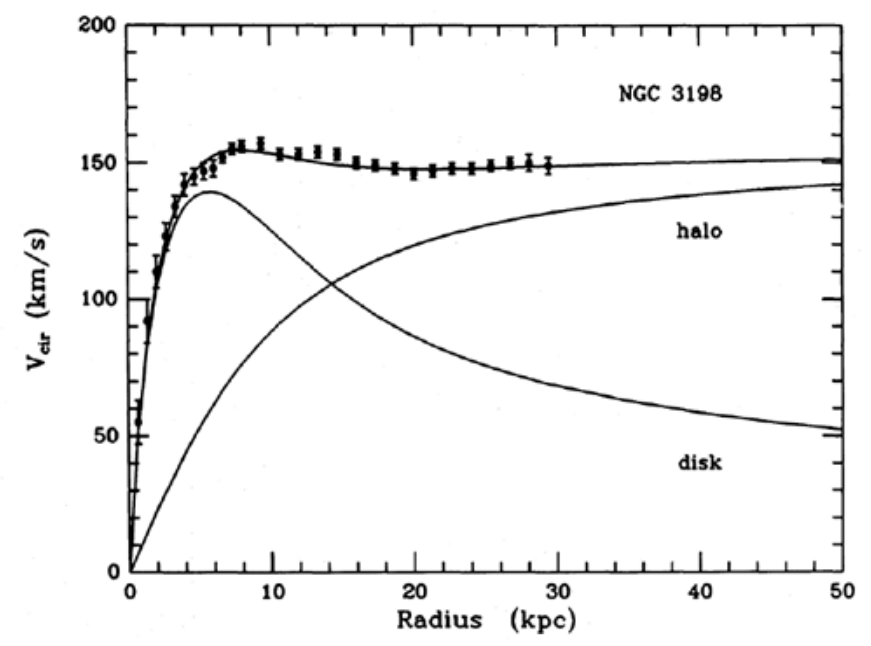
\includegraphics[width=.9\textwidth]{antecedentes/figures/vprofile.png}
    \caption{\label{fig:ejemplo_vpc} Curva de velocidad de rotación de una galaxia espiral barrada \citep{van1985distribution}}.
\end{figure}

\subsection{Atípicos/Outliers}

Otro experimento de interés es la posibilidad de eliminar valores atípicos \textit{outliers}. Estos valores son extremadamente raros o pueden suceder de algún tipo de error de medición. Además, en el contexto de simulaciones hidrodinámicas podemos considerar atípicos a valores que están muy alejados del centro galáctico y puede que estén muy débilmente ligados gravitacionalmente.

Así, hemos decidido utilizar dos métodos para la eliminación de atípicos para probar cómo se comportan los diferentes algoritmos de clustering: uno algorítmico y otro propio de la astronomía.

\subsubsection{\acrfull{IF}}

\citet{liu2008isolation} Detecta anomalías mediante árboles binarios. Divide el espacio de datos mediante líneas paralelas a la base canónica y asigna puntuaciones de anomalía a los datos, como se puede ver en la Fig~\ref{fig:isolation-forest-example}. Otorgando de esta manera valores más altos a los puntos de datos que necesitan menos divisiones para ser aislados.

Para aislar un punto del resto de los datos, el algoritmo genera recursivamente particiones en la muestra seleccionando aleatoriamente un atributo, para luego seleccionar también de forma aleatoria un valor de partición entre los valores mínimo y máximo permitidos por ese atributo.


\begin{figure}
    \centering
    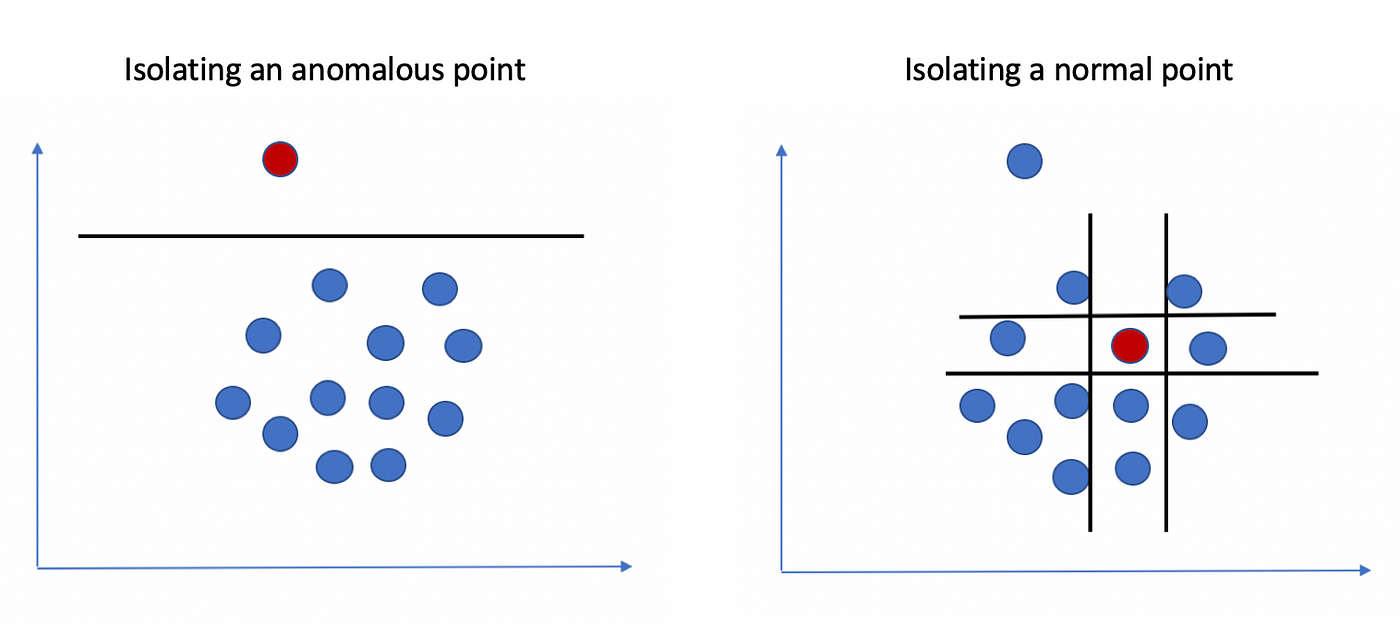
\includegraphics[width=.9\textwidth]{antecedentes/figures/isolation_forest.png}
    \caption{\label{fig:isolation-forest-example} Aislando un punto anómalo en un conjunto de puntos utilizando \gls{IF}. Gráfico proveído por \href{https://towardsdatascience.com/how-to-perform-anomaly-detection-with-the-isolation-forest-algorithm-e8c8372520bc}{Towards Data Science}.}
\end{figure}

En el contexto del problema a tratar en este trabajo, dicho método será aplicado sobre las coordenadas en el espacio real de cada partícula estelar, en lugar de utilizar los parámetros de circularidad descritos anteriormente. Para, de esta manera, intentar identificar las partículas alejadas del centro de la galaxia como se mencionó.

\subsubsection{\acrfull{RCUT}}

Desde el punto de vista de la astrofísica, es habitual considerar a las galaxias como las partículas estelares con radio $r <= X \mathrm{kpc}$, donde kpc es una medida de distancia igual a 3260 años luz y $X$ es 3 veces el radio que encierra la mitad de la masa estelar. Esta heurística es usada en diversos trabajos como una forma rápida de descartar valores que es poco probable que pertenezcan a la galaxia, pero que el algoritmo que identifica las galaxias las haya asignado allí. Puede apreciarse el resultado de utilizar dicho método en la Fig~\ref{fig:rcut-example}.

\begin{figure}
    \centering
    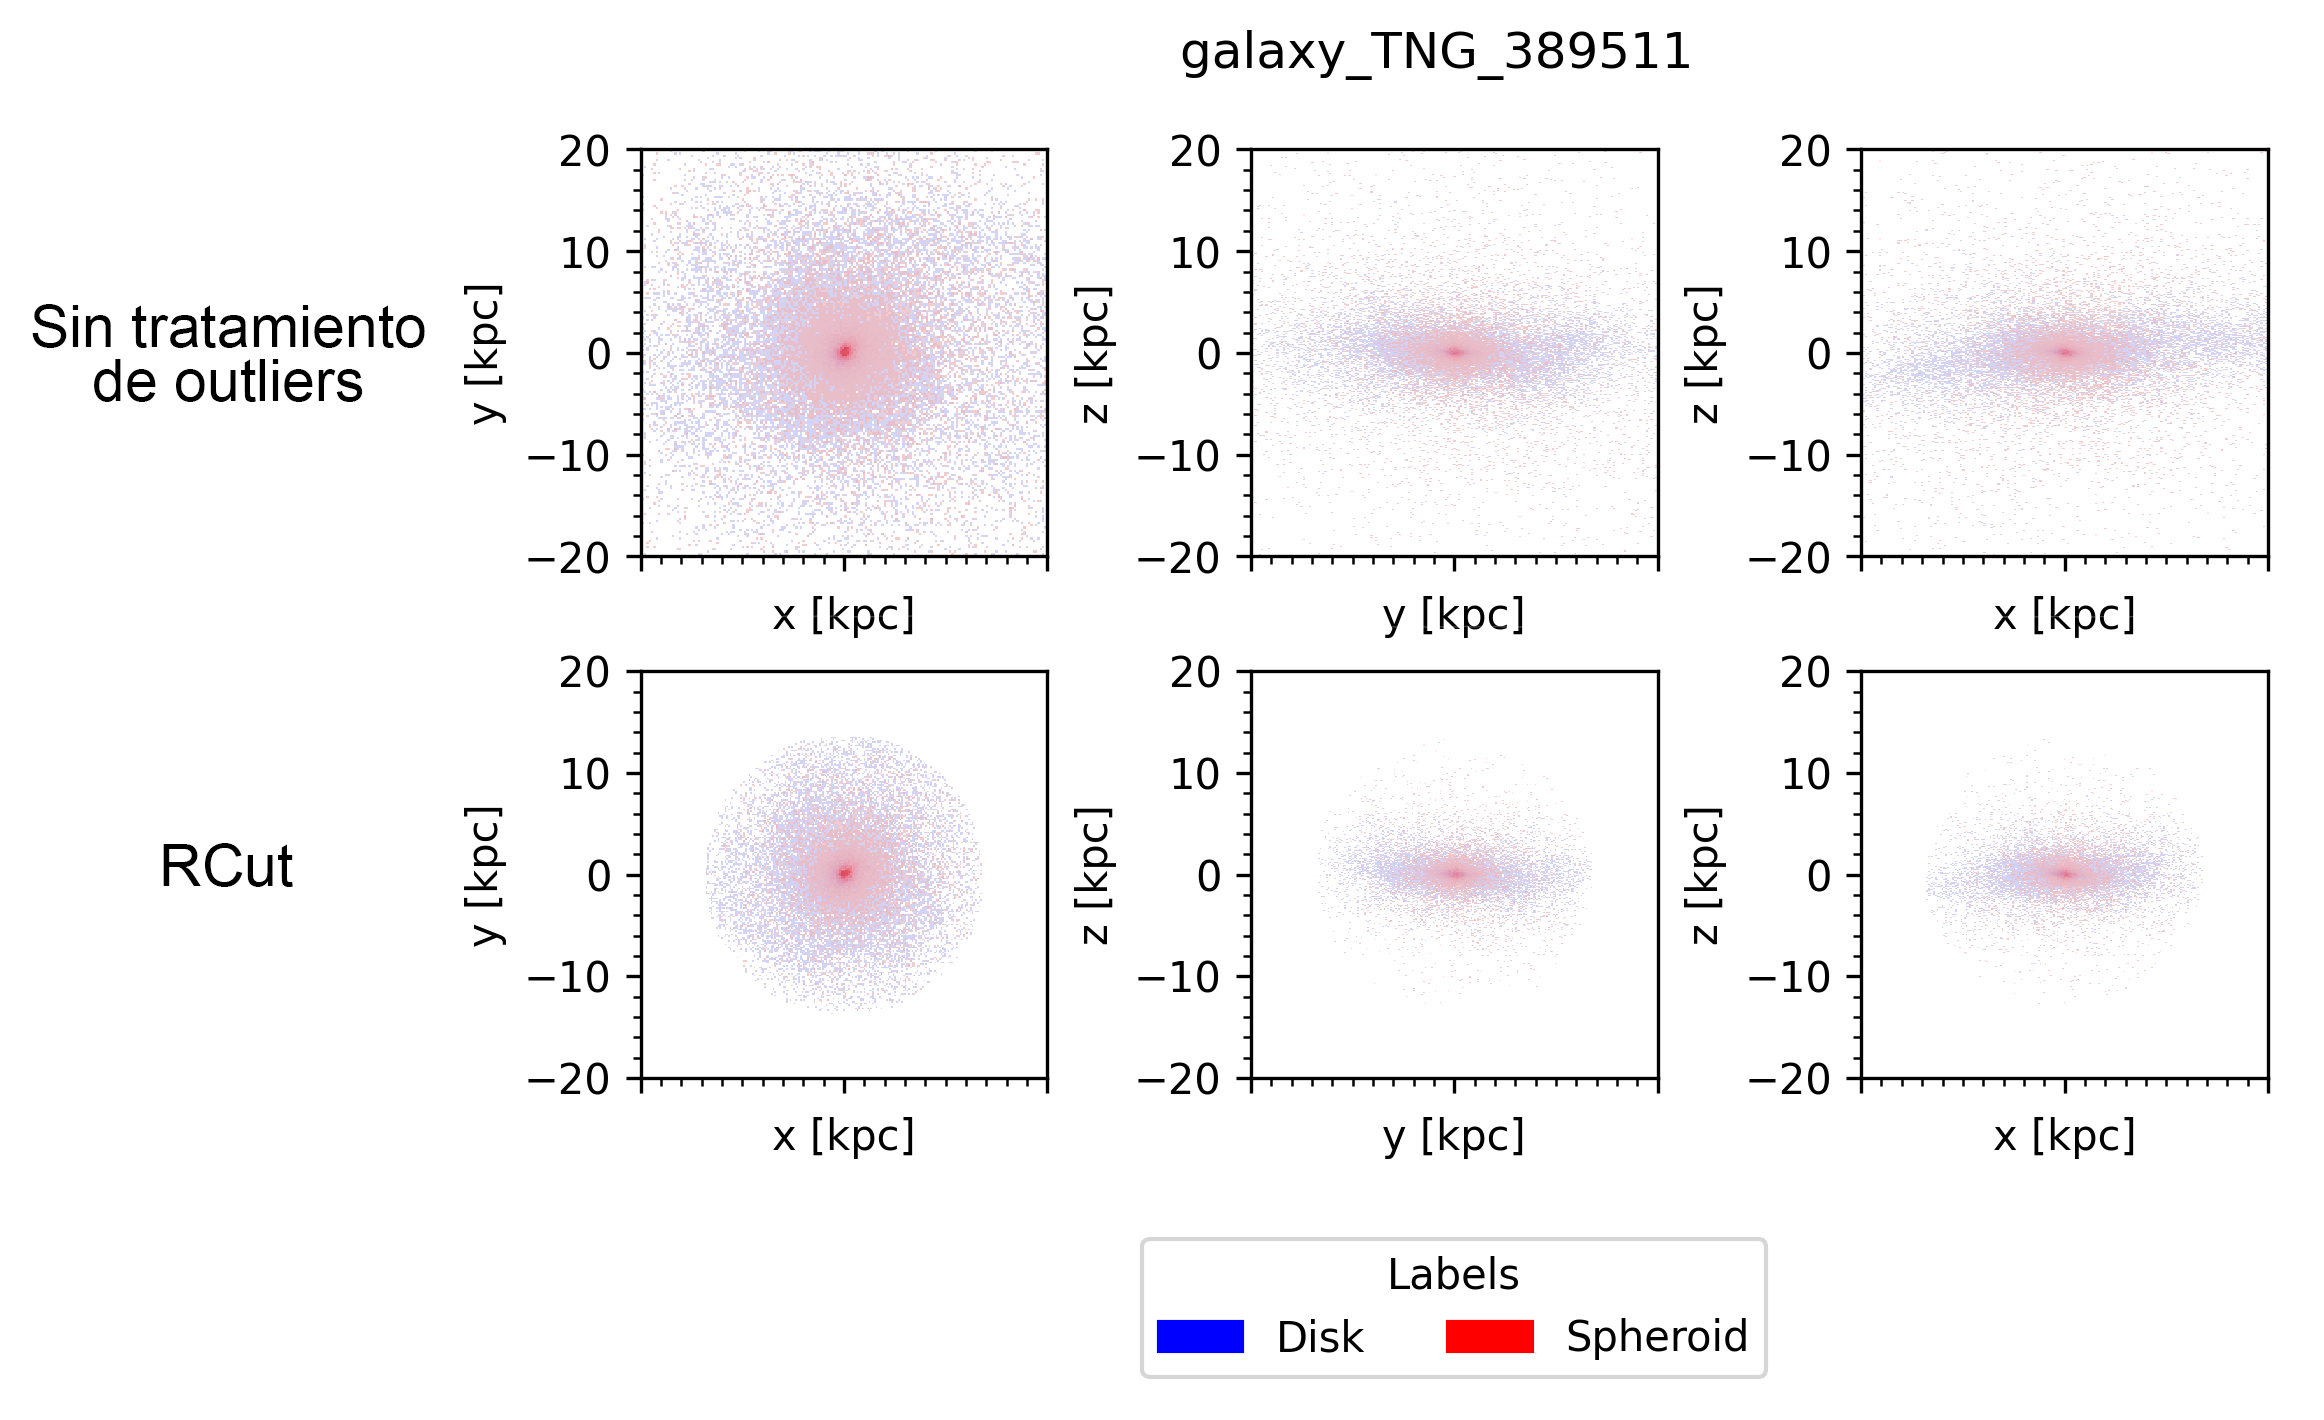
\includegraphics[width=.9\textwidth]{antecedentes/figures/rcut_in_real_space.png}
    \caption{\label{fig:rcut-example} Demostración de \gls{RCUT} sobre la galaxia \textit{galaxy\_TNG\_389511} en espacio real.}
\end{figure}